\documentclass[dvipsnames]{article}
\usepackage{amsmath, amsthm, amssymb, framed, geometry, mdframed, pgfplots, subcaption, tikz} 
\geometry{scale=0.7}
\pgfplotsset{compat=1.18}

\usepackage{tcolorbox}
\tcbuselibrary{skins}

\numberwithin{equation}{section}
\newcounter{problemcounter} % Define a new counter

\newtcolorbox{problem}[1]{%
    enhanced,
    colback=yellow!10!white,
    colframe=OliveGreen,
    fonttitle=\bfseries,
    title={Problem \refstepcounter{problemcounter}\theproblemcounter #1}, % Use the counter in the title
    attach boxed title to top left={yshift=-3mm,xshift=3mm},
    boxed title style={size=small,colback=OliveGreen!50!white}
}



\newtheorem{Theorem}{Theorem}[section] % "Theorem 1.1", "Theorem 2.1", ...
\newtheorem{Lemma}[Theorem]{Lemma}     % Same numbering as Theorem, i.e., "Lemma 1.2", "Lemma 2.2", ...
\newtheorem{Corollary}[Theorem]{Corollary} 
\newtheorem{Definition}[Theorem]{Definition} 
\newtheorem{Remark}[Theorem]{Remark}   
\newtheorem{Example}[Theorem]{Example} 


\newcommand{\Rn}{\mathbb{R}^{n}}



\begin{document}
\large



\section{Introduction}

\subsection{Limit}
Let's first show the process of limit by approximating a real number by $\{k/2^{m}\}$.
\begin{Example}
    Given $x=\sqrt{2}/2$, we search the nearest dyadic number from $m=1$ to $\infty$. Notice that we just need consider $1/2^{m}$ because $2/2^{m}=1/2^{m-1}$ is supposed to be added before.
    \begin{enumerate}
        \item $m=1$, there is $1/2<x$ and we denote $x-1/2$ by $x_{1}$.
        \item $m=2$, $1/4>x_{1}$ and we enter next $m$.
        \item $m=3$, $1/8<x_{1}$ and we denote $x_{1}-1/8$ by $x_{2}$,
        \item continue...
    \end{enumerate}
\end{Example}
Thanks to the countable property of $k/2^{m}$, we can continue this procedure and have
$$
\frac{\sqrt{2}}{2}=1/2+1/8+\cdots
$$
One can view this as decomposition of open interval $(0,x)$ or any interval with length $x$ by shifting for need. More general, we have
\begin{Theorem}
    Every open set $U$ in $\Rn$ can be written as a countable union of almost disjoint cubes.
\end{Theorem}

\begin{proof}
Consider the collection of all cubes in $\mathbb{R}^n$ whose vertices have coordinates of the form $k/2^m$, where $k\in\mathbb{Z}, m\in\mathbb{N}^{*}$. Denote these dyadic cubes by 
$$
A_{m}= \{(x_1, x_2, \cdots, x_{n})\in\mathbb{R}^{n}, \frac{k_i}{2^m}\leq x_{i} <\frac{k_i+1}{2^{m}}\;\text{for}\; i=1,2,\cdots, n\}
$$ 

For fixed $m$, $A_{m}$ is countable since it's determined by $(k_1, k_2,\cdots, k_{n})\in\mathbb{Z}^{n}$. Therefore $\mathcal{A}:=\cup_{m} A_{m}$ is also countable and we create an enumeration $D_{1}, D_{2},\cdots$. 

Last, we show how to select a sub-collection from $\mathcal{A}$ to satisfy $U = \cup D_{j}$. 
Let $U$ be an open set in $\mathbb{R}^n$. For each $x \in U$, since $U$ is open, there exists a dyadic cube containing $x$ and fully contained within $U$.

\begin{enumerate}
    \item We start with an empty collection, and then iterate through the dyadic cubes contained in $U$

    \item For each cube, if it is almost disjoint from every cube already in our collection, we add it.
    \begin{center}
    \begin{figure}[ht]
\label{plot2}
    \centering
    \begin{subfigure}[b]{0.3\textwidth}
        \centering
        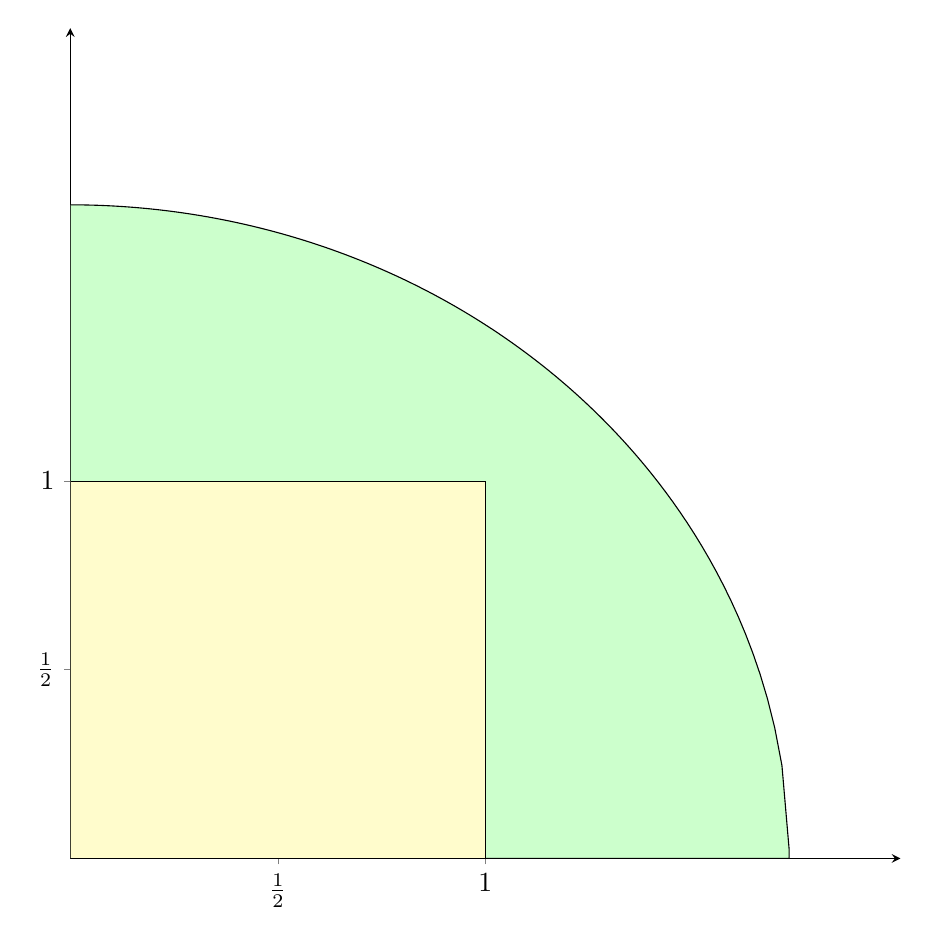
\begin{tikzpicture}
            \begin{axis}[axis lines=middle, 
            xmin=0, xmax=2, 
            ymin=0, ymax=2.2, 
            width=\textwidth, height=\textwidth,
            xtick={0,0.5,1}, % Adjust x-axis ticks
            xticklabels={0,$\frac{1}{2}$,1}, % Custom x-axis labels
            ytick={0.5,1}, % Adjust y-axis ticks
            yticklabels={$ \frac{1}{2}$,1} % Custom y-axis labels 
            ]
                % Quarter circle
                \addplot[domain=0:1.732, samples=100, fill=green!20] {sqrt(3-x^2)} \closedcycle;
                % First cube
                \addplot[fill=yellow!20] coordinates {(0,0) (1,0) (1,1) (0,1) (0,0)};
                % Second cube
                
            \end{axis}
        \end{tikzpicture}
        \caption{collection $C_{1}$}
    \end{subfigure}
    \hfill
    \begin{subfigure}[b]{0.3\textwidth}
        \centering
        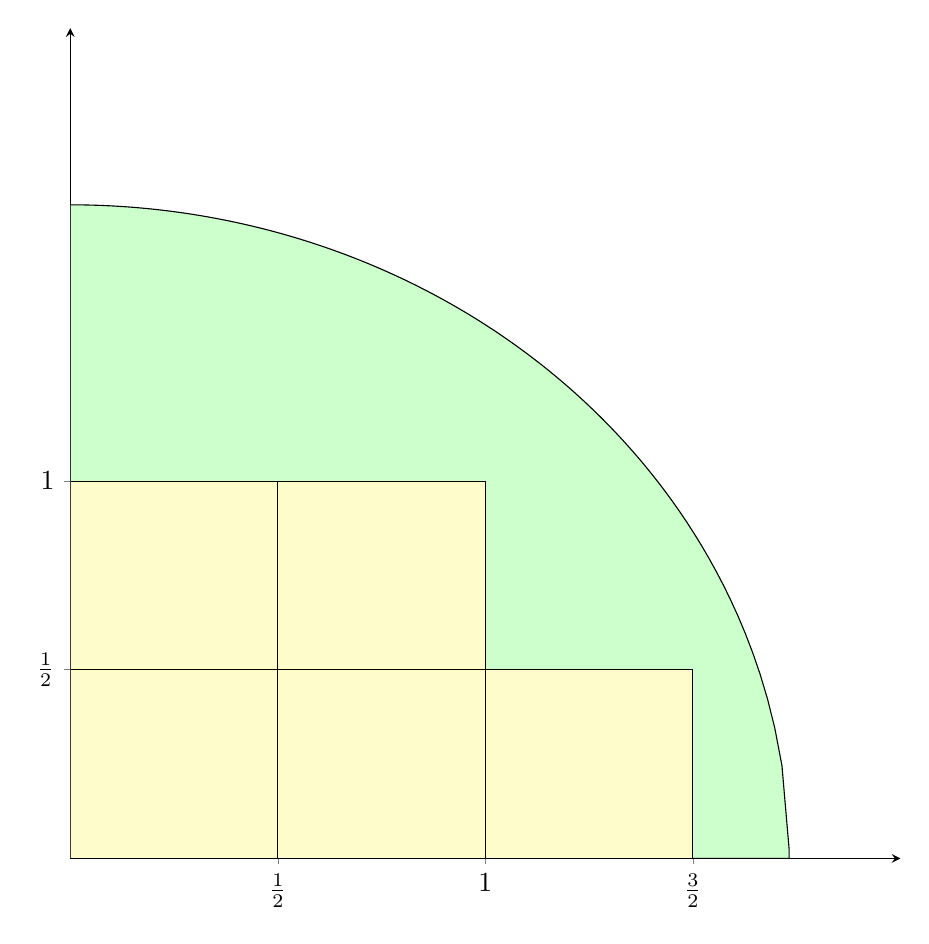
\begin{tikzpicture}
            \begin{axis}[axis lines=middle, 
            xmin=0, xmax=2, 
            ymin=0, ymax=2.2, 
            width=\textwidth, height=\textwidth,
            xtick={0,0.5,1,1.5}, % Adjust x-axis ticks
            xticklabels={0,$\frac{1}{2}$,1,$\frac{3}{2}$}, % Custom x-axis labels
            ytick={0.5,1}, % Adjust y-axis ticks
            yticklabels={$ \frac{1}{2}$,1} % Custom y-axis labels 
            ]
                % Quarter circle
                \addplot[domain=0:1.732, samples=100, fill=green!20] {sqrt(3-x^2)} \closedcycle;
                % Finer cubes
                \addplot[fill=yellow!20] coordinates {(0,0) (0.5,0) (0.5,0.5) (0,0.5) (0,0)};
                \addplot[fill=yellow!20] coordinates {(0.5,0) (1,0) (1,0.5) (0.5,0.5) (0.5,0)};
                \addplot[fill=yellow!20] coordinates {(0,0.5) (0.5,0.5) (0.5,1) (0,1) (0,0.5)};
                \addplot[fill=yellow!20] coordinates {(0.5,0.5) (1,0.5) (1,1) (0.5,1) (0.5,0.5)};
                \addplot[fill=yellow!20] coordinates {(1,0) (1.5,0) (1.5,0.5) (1,0.5) (1,0)};
            \end{axis}
        \end{tikzpicture}
        \caption{collection $C_{2}$}
    \end{subfigure}
    \hfill
    \begin{subfigure}[b]{0.3\textwidth}
        \centering
        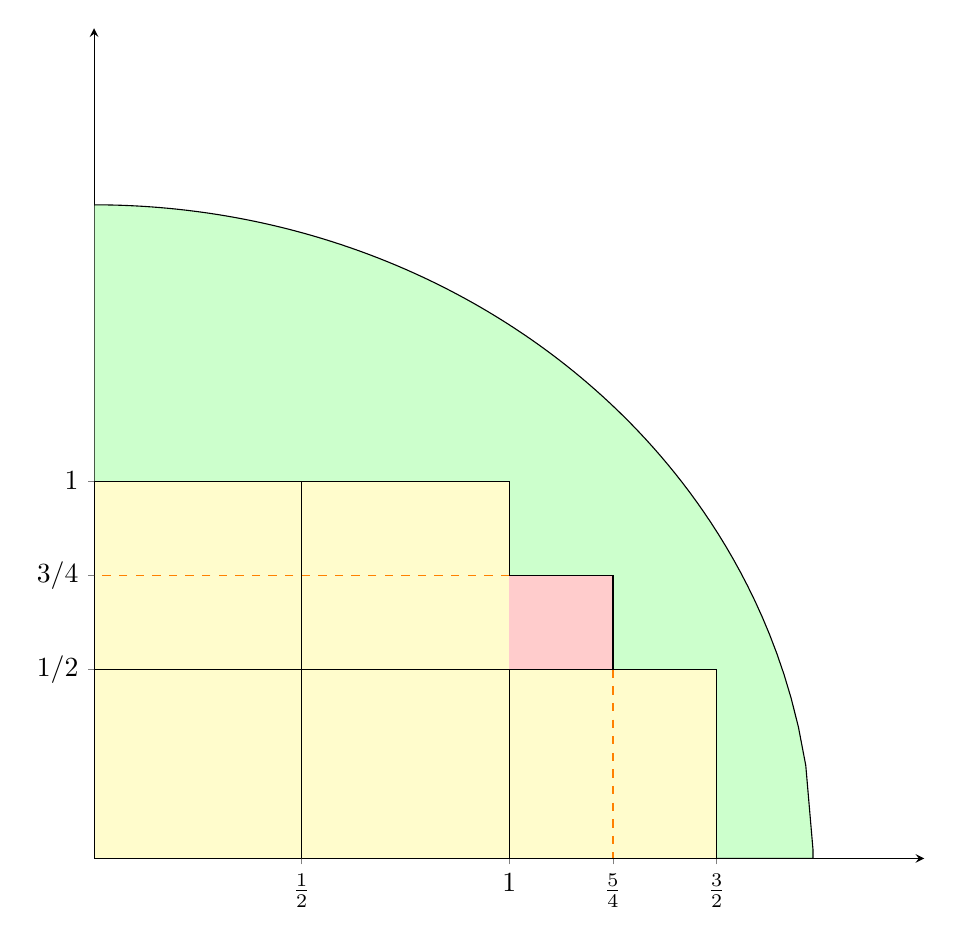
\begin{tikzpicture}
            \begin{axis}[axis lines=middle, 
            xmin=0, xmax=2, 
            ymin=0, ymax=2.2, 
            width=\textwidth, height=\textwidth,
            xtick={0,0.5,1, 1.25, 1.5}, % Adjust x-axis ticks
            xticklabels={0,$\frac{1}{2}$,1, $\frac{5}{4}$, $\frac{3}{2}$}, % Custom x-axis labels
            ytick={0.5, 0.75, 1}, % Adjust y-axis ticks
            yticklabels={$ 1/2$,$3/4$, 1} % Custom y-axis labels 
            ]
                % Quarter circle
                \addplot[domain=0:1.732, samples=100, fill=green!20] {sqrt(3-x^2)} \closedcycle;
                % Finer cubes
                \addplot[fill=yellow!20] coordinates {(0,0) (0.5,0) (0.5,0.5) (0,0.5) (0,0)};
                \addplot[fill=yellow!20] coordinates {(0.5,0) (1,0) (1,0.5) (0.5,0.5) (0.5,0)};
                \addplot[fill=yellow!20] coordinates {(0,0.5) (0.5,0.5) (0.5,1) (0,1) (0,0.5)};
                \addplot[fill=yellow!20] coordinates {(0.5,0.5) (1,0.5) (1,1) (0.5,1) (0.5,0.5)};
                \addplot[fill=yellow!20] coordinates {(1,0) (1.5,0) (1.5,0.5) (1,0.5) (1,0)};
                % Additional cube
                \addplot[fill=red!20] coordinates {(1,0.5) (1.25,0.5) (1.25,0.75) (1,0.75)};
                \addplot[orange, dashed] coordinates {(1.25, 0.5) (1.25, 0)};
                \addplot[orange, dashed] coordinates {(1, 0.75) (0, 0.75)};
            \end{axis}
        \end{tikzpicture}
        \caption{collection $C_3$}
    \end{subfigure}
    \caption{We use dyadic square to approximate the quarter. Note that the sub-collection is not unique since we can choose 4 smaller quads in place of 1-by-1 quad. This process can be viewed as 2D-version of determining series $\{a_{n}\}\in \mathbb{Z}^{n}$ such that $x=\sum a_{n}/2^{n}$ for any real number $x$.}
\end{figure}
    \end{center}
\end{enumerate}
Since $\mathcal{A}$ is countable, the sub-collection we get is also countable.
\end{proof}

\subsection{Limit of sets}

One advantage of Lebesgue measure is to deal with some special set which is a limit of a collection of sets. For example,
$(0,1) \cap \mathbb{Q}$ can be viewed as an infinite union of set
$$
E_{k} = \left\{\frac{m}{k}: \operatorname{gcd}(m,k)=1, m<k \right\}.
$$

More interesting and important sets are
$$
\bigcap_{i=1} \bigcup_{k=i}^{\infty} A_{k}
$$
and
\begin{equation}
\label{basic_set2}
    \bigcup_{i=1} \bigcap_{k=i}^{\infty} A_{k}
\end{equation}
which represents "elements appeared in $A_{k}$ for infinite $k$" and "elements appeared in $A_{k}$ for all but finite $k$" respectively.

For example, we can reinterpret the set of points where $f_{k}(x)$ converges to $f(x)$ pointwise into
\begin{equation}
    \label{pointwiseSet}
    \bigcap_{n=1} \boxed{\bigcup_{i=1} \bigcap_{k\geq i} \left\{x: |f_{k}(x)-f(x)|<\frac{1}{n}\right\}}
\end{equation}
Notice that the boxed part is exactly interpretation of "for all $k\geq K(n, x)$, we have..." when $n$ (or $\varepsilon$) is given. In other words, it's those points that can appear in all but finite $A_{k,n}$, where $n$ can be seen as a additional parameter to eq~\eqref{basic_set2} 

And the set whose point is uniform convergent is 
\begin{equation}
\label{uniformSet}
    \bigcap_{n=1} \boxed{\bigcap_{k\geq K(n)} \left\{x: |f_{k}(x)-f(x)|<\frac{1}{n}\right\}}.
\end{equation}
The essence of Egoroff theorem lies in 
\begin{equation}
\label{eq_critical2Egoroff}
    \lim_{K\to \infty} \mu\left(\bigcup_{k\geq K} \left\{x: |f_{k}(x)-f(x)|\geq \frac{1}{n}\right\}\right) = 0
\end{equation}
due to \eqref{pointwiseSet} and \textbf{finite measure} of $X$. In detail, since 
\begin{equation}
    \label{eqD}
    \mu\left(\bigcap _{i\geq 1} \bigcup_{k\geq i} \left\{x: |f_{k}(x)-f(x)|\geq \frac{1}{n}\right\}\right) = 0,
\end{equation}
which implies $\bigcup_{k\geq i} \left\{x: |f_{k}(x)-f(x)|\geq \frac{1}{n}\right\}$ are shrinking to a null set and we can control it to a small size saying $\varepsilon/2^n$ by terminating at $K_{n, \varepsilon}$-th step.

\begin{Remark}
    We must have $\mu(X)<\infty$ to deduce eq\eqref{eq_critical2Egoroff} from \eqref{eqD}, i.e. we can apply
    $$
    \lim_{n\to\infty} \mu(A_{i}) =\mu(\cap A_{i}) = 0
    $$
    to a descending set $A_{i}$ only if $\mu(X)<\infty$. For instance,
    
    \vspace{0.4cm}
    \fbox{\begin{minipage}{30em}
        \centering
        $f_{k}(x) = \chi_{[k,k+1]}$ and $f_{k}\to 0$ pointwisely in $\mathbb{R}$.
    \end{minipage}}
    
    \vspace{0.4cm}
\end{Remark}

\begin{Theorem}
    If $\{f_{k}\}$ converges to $f$ in measure, one can find a subsequence $f_{k_{j}}$ such that $f_{k_j}\to f$, a.e.
\end{Theorem}

\begin{proof} We give a construction about subsequence by diagonal principle. We aim to prove there exists a subsequence $\{f_{k_j}\}$ satisfying
\begin{equation}
\label{eq_measure2pw}
    \mu\left(\bigcap _{i= 1}^{\infty} \bigcup_{j\geq i} \left\{x: \boxed{|f_{k_j}(x)-f(x)|\geq \frac{1}{n}}\right\}\right) = 0,\;\forall n,
\end{equation}
Claim: $\{f_{k_j}\}$ satisfying
$$
\mu\left(\bigcup_{j\geq i} \left\{x: \boxed{|f_{k_j}(x)-f(x)|\geq \frac{1}{i}}\right\}\right) = \frac{1}{i}, \;\forall i
$$
is eligible for eq\eqref{eq_measure2pw}.

View $1/i$ as $\varepsilon$, we decompose $\varepsilon$ as $\sum \varepsilon/2^{j}$ and determine $f_{i,k_1}, f_{i,k_2},\cdots, f_{i,k_n}$ such that 
\begin{equation}
\label{condition1}
    \mu\left(\{x: |f(x)-f_{i,k_j}(x)|\geq 1/i\}\right) \leq \frac{\varepsilon}{2^j}.
\end{equation}


If we use $f_{i,n}$ in place of $f_{i,k_n}$ for simplicity, we can pick the diagonal element as desired subsequence.
$$
\begin{array}{cccccc}
    \boxed{f_{1,1}} & f_{1,2} & f_{1,3} & \cdots & f_{1,n} & \cdots\\
    f_{2,1} & \boxed{f_{2,2}} & f_{2,3} & \cdots & f_{2,n} & \cdots\\
    f_{3,1} & f_{3,2} & \boxed{f_{3,3}} & \cdots & f_{3,n} & \cdots\\
    \vdots  & \vdots  & \vdots  &    &   \vdots&\\
    f_{n,1} & f_{n,2} & f_{n,3} & \cdots & \boxed{f_{n,n}} & \cdots
\end{array}
$$
\end{proof}

\textit{Proof of Claim.} Note that 
$$
\begin{aligned}
    {\color{blue}\bigcap _{i= 1}^{\infty}} \bigcup_{j\geq i} \left\{x: \boxed{|f_{k_j}(x)-f(x)|\geq \frac{1}{n}}\right\} 
    &\subset 
    {\color{red}\bigcap _{i= n}^{\infty}} \bigcup_{j\geq i} \left\{x: \boxed{|f_{k_j}(x)-f(x)|\geq \frac{1}{n}}\right\}
    \\
    &\subset 
    \bigcap _{i= n}^{\infty} \bigcup_{j\geq i} \left\{x: \boxed{|f_{k_j}(x)-f(x)|\geq \frac{1}{i}}\right\}
\end{aligned}
$$
and 
$$
B_{i}:= \bigcup_{j\geq i} \left\{x: \boxed{|f_{k_j}(x)-f(x)|\geq \frac{1}{i}}\right\}
$$
is descending sequence with measure less than $1/i$. To ensure the validity of 
$$
\mu\left(\bigcap_{i=1}^{\infty}B_{i}\right) {\color{blue}=} \lim_{i}\mu(B_{i}) =\lim_{i} 1/i=0
$$
it suffices to show that $\mu(B_1)<\infty$. Actually, $\mu(B_1)\leq 1$ due to our condition~\eqref{condition1}.

\end{document}